\documentclass[no]{./../../common/SurferDesc}%%%%%%%%%%%%%%%%%%%%%%%%%%%%%%%%%%%%%%%%%%%%%%%%%%%%%%%%%%%%%%%%%%%%%%%
%
% The document starts here:
%
\begin{document}
\footnotesize
% Weltrekordfl�chen

%%% 1.Tafel

%%%%%%%%%%%%%%%%%%%%%%%%%%%%%


\begin{surferPage}
  \begin{surferTitle}En 7-gon-symmetrisk flate av sjuende grad\end{surferTitle}   \\
  
Denne flaten, som ligner p� en stjerne, er av sjuende grad og har $84$ singulariteter. Inntil nylig var det ikke kjent om en flate av sjuende grad kunne ha flere reelle singulariteter, men i 2004 forbedret Oliver Labs denne verdensrekorden til $99$. 
  
  
 De tre putene som ligger over hverandre ved flaten p� det store bildet, er der p� grunn av de s�kalte Chebychev-polynomene. De ligner de du kan finne p� Chmutov-flaten av �ttende grad, og faktisk er denne stjerneformede flaten en variant av Chmutovs flater. Her er den plane kurven $T_d(x)+T_d(y)$ erstattet med en vanlig $7$-gon  $S_7(x,y)$: 
   \[S_7(x,y) + \lambda \cdot T_d(z) = 0,\]
   for en passende valgt $\lambda\in\RR$. 
    \vspace*{-0.3em}
    \begin{center}
      \begin{tabular}{c@{\qquad}c}
        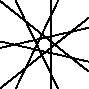
\includegraphics[height=1.5cm]{./../../common/images/labsseptic1.pdf}
        &
        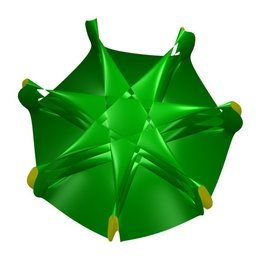
\includegraphics[height=1.5cm]{./../../common/images/septic_7eck_von_oben}
      \end{tabular}
    \end{center}
    \vspace*{-0.3em}   
   Denne varianten av Chmutovs konstruksjon er utviklet av Duco van Straten. 


  \begin{surferText}
     \end{surferText}
\end{surferPage}



\end{document}
%
% end of the document.
%
%%%%%%%%%%%%%%%%%%%%%%%%%%%%%%%%%%%%%%%%%%%%%%%%%%%%%%%%%%%%%%%%%%%%%%%
